\chapter{Sistem de dialog}

Construcția unui agent virtual menit să întrețină cursul unei conversații a fost întotdeauna un etalon al performanței de cercetare, de aceea testul ce poartă numele cercetătorului britanic Allan Turing \ref{test-turing} a fost pană de curând un criteriu în această direcție.

Au fost propuse diferite arhitecturi și moduri de a schița matematic o conversație, printre ele și ELIZA compus dintr-un set de reguli elaborate pe baza mai multor studii având la bază logica. Bineînțeles industria cere și abordări mai modulare, mai robuste dar care să nu iasă din tipare, în această speță făcândi-și apariția prima arhitectură bazată pe umplerea de sloturi (GUS), adică pentru fiecare replică din dialog se extrag constituenți semantici specifici domeniului care mai apoi sunt completați într-o structură tabelară (frame) urmând să servească drept parametrii în interogările cu sistemul.

Dacă privim la scopul final al unei conversații distingem două clase și anume: agenți orientați pe rezolvarea de cerințe și agenți orientați pe discuție la nivel general.

Din categoria sistemelor de dialog ce au ca scop rezolvarea de cerințe 


\section{Înțelegerea limbajului natural}
NLU este un concept destul vast, in terminologia sistemelor de dialog acesta joacă rolul componentei care detectează intenția vorbitorului si extrage constituenți semantici din limbajul natural exprimat.
Detecția intenției poate fi tratata ca o problema de clasificare a unei replici din punct de vedere semantic, iar recunoașterea entităților poate fi văzută ca o etichetare de secvențe.
\subsection{Abordări anterioare}
Pentru detectarea intenției se pot folosi tehnici standard de clasificare a unui text si anume SVM (Haffner et al., 2003), dar si rețele neurale convoluționale (CNNs) (Xu and Sarikaya, 2013) întâlnite adesea în procesarea imaginilor.

Pentru recunoașterea entităților se folosesc abordări precum (MEMMs) (McCallum et al., 2000), conditional random fields (CRFs) (Raymond and Riccardi, 2007), și rețele neurale recurente (RNNs) (Yao et al., 2014; Mesnil et al., 2015)

Având la baza înțelegerea limbajului, majoritatea lucrărilor recente se concentrează pe rezolvarea concomitenta a acestor doua probleme, întrucât combinarea celor doua modele ajuta la învățarea unei reprezentări cat mai precise a textului.



\subsection{Seq2Seq}

\begin{figure}[h]
	\centering
	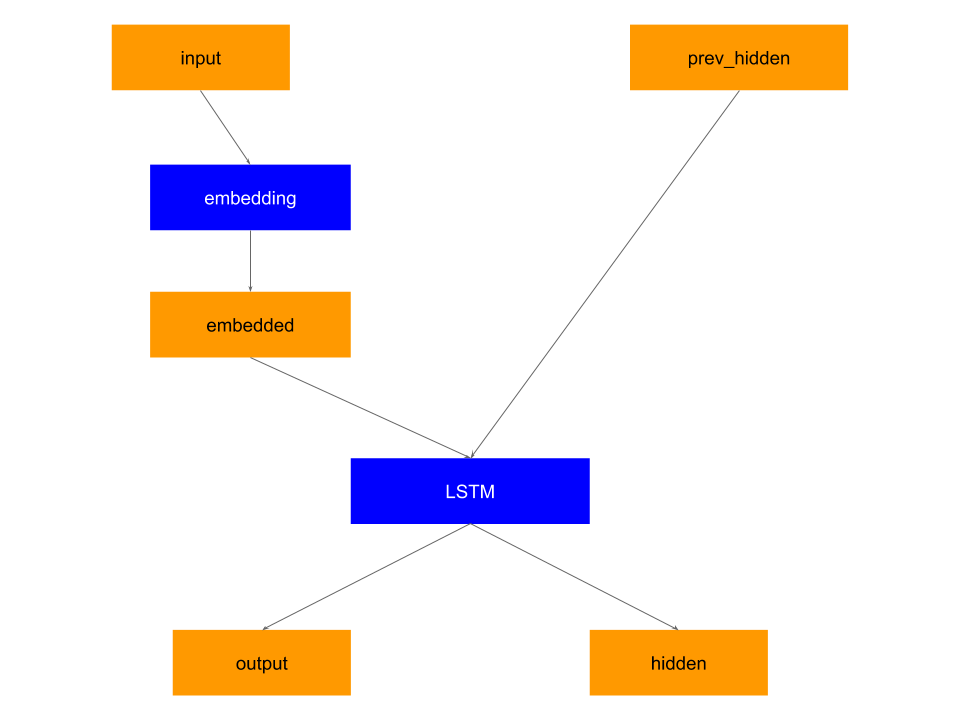
\includegraphics[scale=0.35]{encoder_module.png}
	\caption{Bidirectional Encoder}
	\label{fig:enc_module}
\end{figure}


\begin{figure}[h]
	\centering
	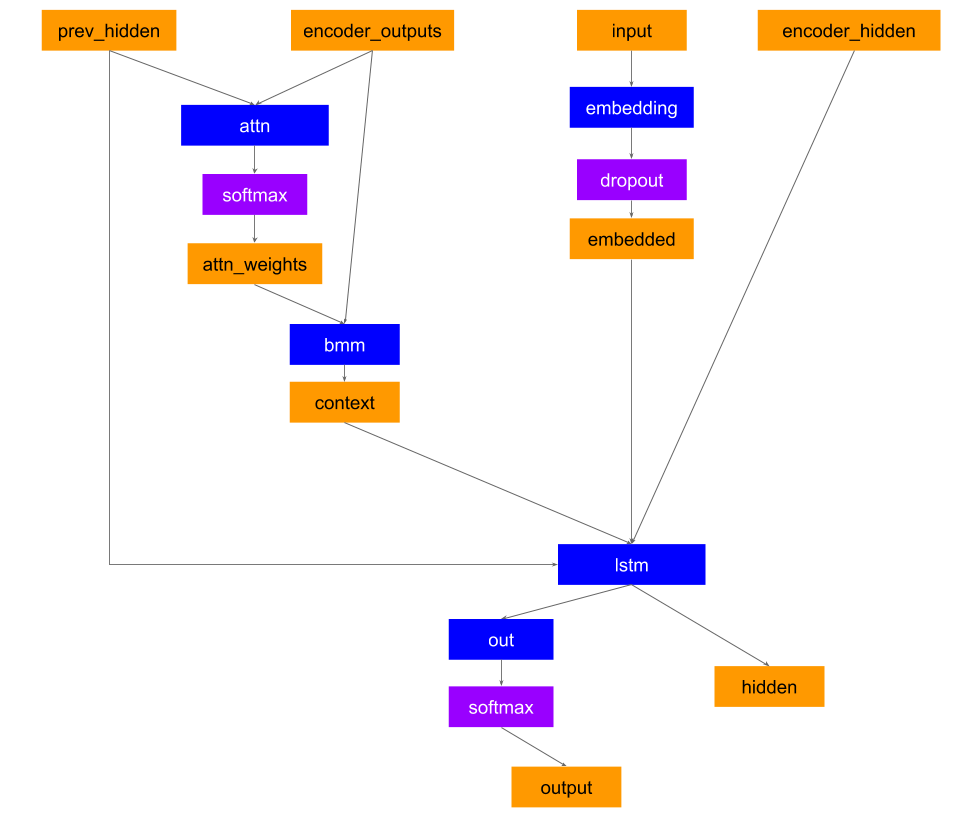
\includegraphics[scale=0.35]{decoder_bahdanau.png}
	\caption{Decoder Bahdanau}
	\label{fig:dec_bah}
\end{figure}

\section{Administrator de dialog}

\subsection{Abordări anterioare}

\subsection{Slot filling}

\section{Metode de evaluare}

\section{Rezultate}